\section{Caratteristiche del navigatore}
\label{sec:chapter_navigazione_scena_caratt_navigat}

Il navigatore offre una interfaccia grafica grazie alla quale l’utente è in grado di fruire una scena fotorealistica.
\\
In particolare permette all’utilizzatore di caricare la scena e di scegliere la modalità di navigazione che preferisce tra: visione dall’alto e visione in prima persona. 
Inoltre, in ogni momento, risulta possibile cambiare la modalità e rimuovere la scena, importandone una nuova.
\\
La navigazione in prima persona rappresenta la funzionalità principale del servizio e gran parte dello sviluppo è stato richiesto per essa.
Quando viene avviata, risulta possibile consultare una mappa di navigazione che mostra l’ ambiente da una vista aerea.
\\
In particolare la mappa di navigazione mostra i movimenti e l’orientamento dell’osservatore, all’interno dell’ambiente, tramite un indicatore che viene modificato in tempo reale. 
Permette infatti all’utilizzatore di orientarsi all’interno della scena ed è particolarmente utile in ambienti di medie e grandi dimensioni.
\\
Il navigatore permette l’utilizzo di differenti tipologie di mappe, che verranno descritte nel paragrafo \ref{sec:caratteristiche_navigatore_mappa}.
Infine il servizio permette di passeggiare all’interno della scena creata tramite una vista stereoscopica sfruttando i visori per la realtà virtuale. 
\\
La scena in questa modalità risulta visibile in 3D dando all’utilizzatore l’idea di trovarsi veramente all’interno di essa.
Questo tipo di tecnologie hanno preso progressivamente piede negli ultimi anni, mostrando potenzialità crescenti nell’ambito dell’intrattenimento, professionale ed educativo.
Il mercato di questi prodotti è in espansione e gli investimenti su nuove tecnologie virtuali o di applicazioni basate su esse sono aumentate esponenzialmente. 
\\
In questo lavoro di tesi sono state sperimentate queste tecnologie, in particolare i sensori di realtà virtuale, al fine di valutarne la precisione ed il grado di realismo permesso. 
In dettaglio è stato valutato quanto queste tecnologie riescano ad immergere l’utilizzatore all’interno delle scena fotorealistiche create, dandogli l’illusione di trovarsi fisicamente all’interno di esse.

\subsection{Navigazione dall' alto ed in prima persona}
\label{sec:chapter_navigazione_scena_caratt_navigat_navig_alto}
Il servizio di navigazione offre all’utente, una volta caricata la scena, di scegliere tra due differenti modalità: navigazione dall’alto o navigazione in prima persona.
\\
La prima modalità permette di osservare la scena dall’alto e di interagire con essa muovendo la camera nella direzione desiderata o zoomando su di essa. 
\\
Il volume di vista può essere modificato tramite l’utilizzo del mouse, del trackpad o del touch screen nel caso in cui venga utilizzato uno smartphone/tablet.
In questa modalità viene utilizzata una camera prospettica, descritta nel paragrafo \ref{sec:chapter_stato_arte_rendering_pipeline}. 
\\
Questa permette di osservare la scena in modo simile a come si farebbe nella vita reale, con gli oggetti che diventano mano a mano più piccoli all’allontanarsi dall’osservatore.
\\
\begin{figure}[htb]
 \centering
 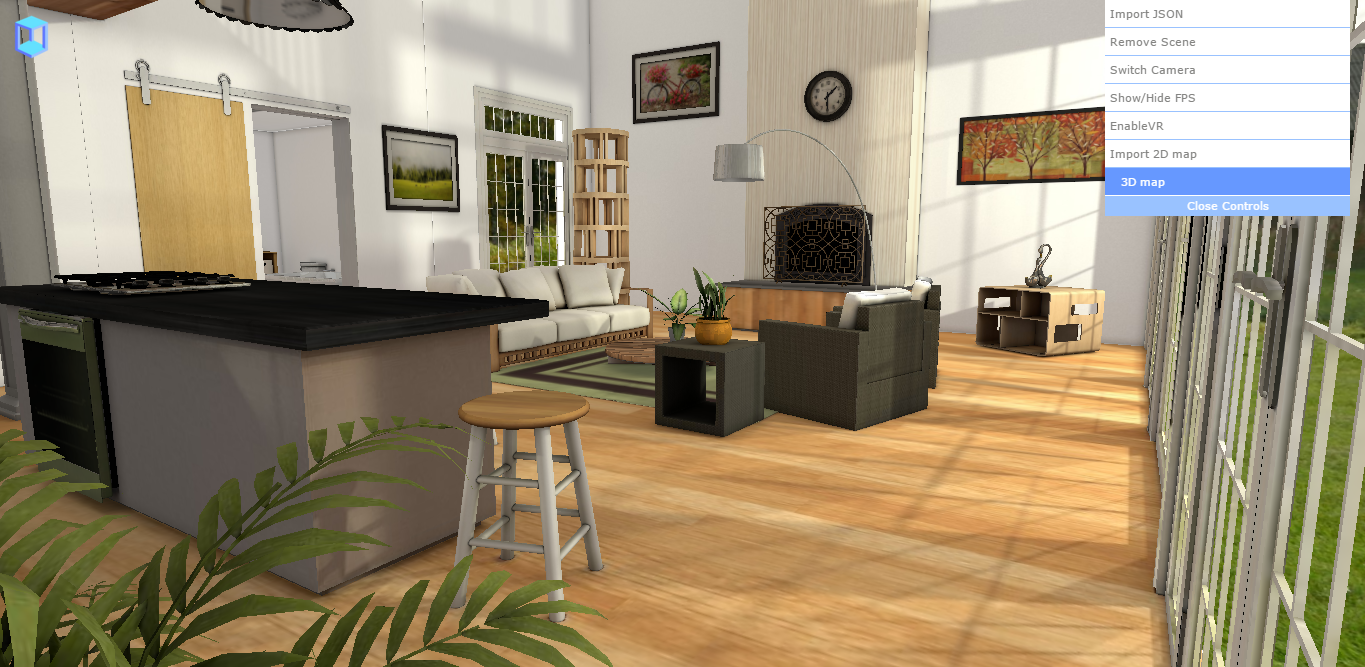
\includegraphics[width=1\linewidth]{images/chapter_navigazione_scena/navigator_persp.png}\hfill
 \caption[Navigazione in prima persona]{Una immagine della navigazione in prima persona.}
 \label{fig:navigazione_scena_navigator_persp}
\end{figure}
\\
Questa modalità permette all’utente di avere una visione completa dell’ambiente realizzato. Inoltre l’utente può modificare la camera a proprio piacimento, permettendogli di osservare ogni dettaglio della scena.
In particolare la vista dall’alto risulta utile, quando viene caricato un appartamento, per osservare la struttura esterna ed interna dell’abitazione creata dall’ angolazione desiderata.
\\
\begin{figure}[htb]
 \centering
 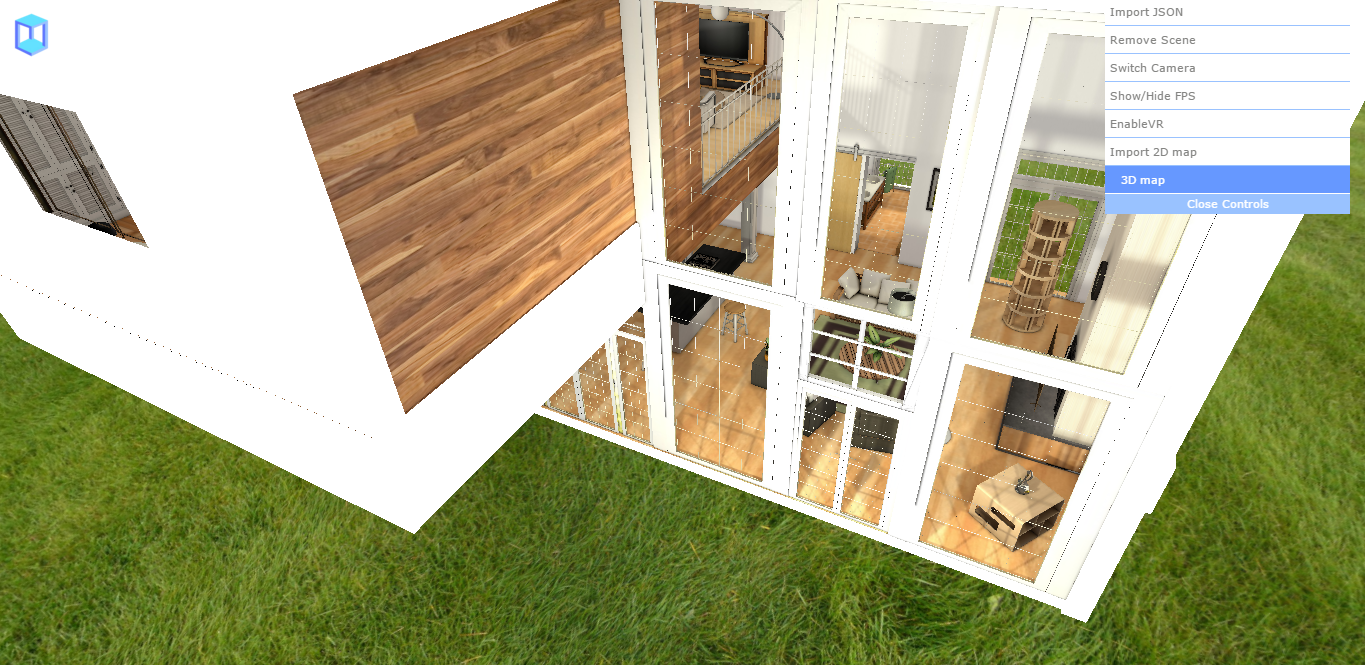
\includegraphics[width=0.96\linewidth]{images/chapter_navigazione_scena/navigator_est.png}\hfill
 \caption[Navigazione dall'alto: veduta esterna]{Una immagine della navigazione in prima persona con veduta esterna dell'abitazione.}
 \label{fig:navigazione_scena_navigator_est}
\end{figure}
\begin{figure}[htb]
 \centering
 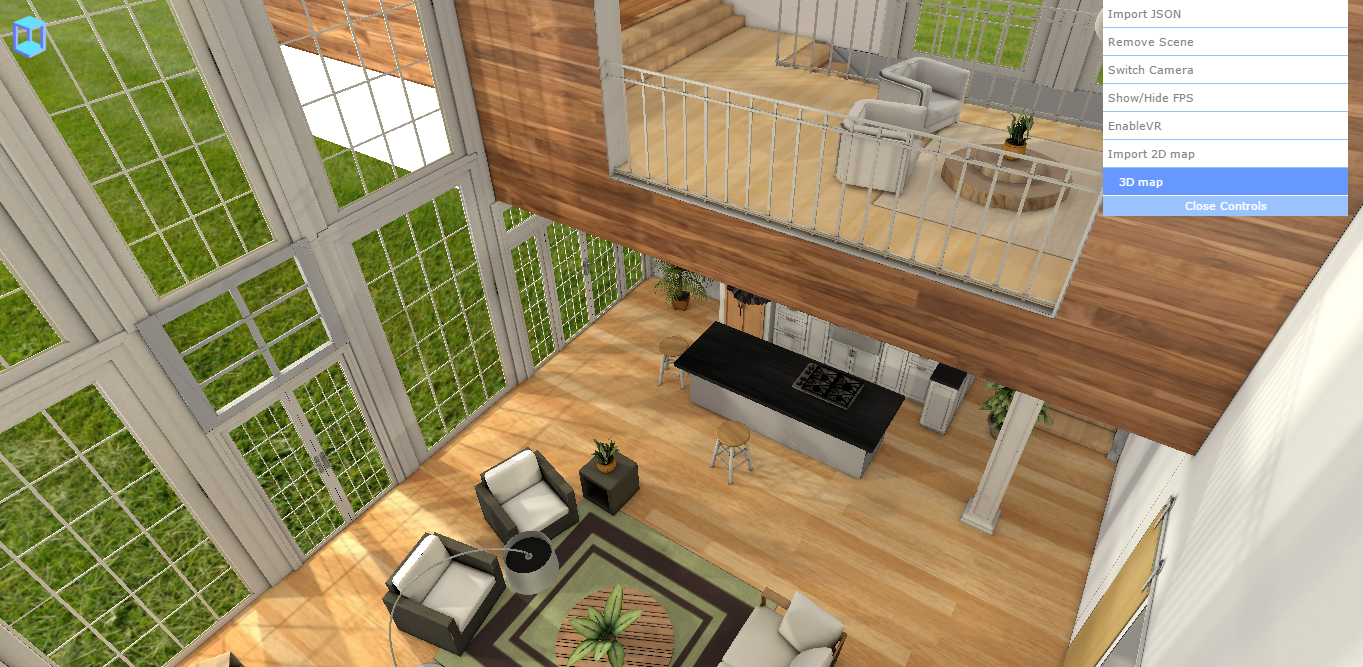
\includegraphics[width=0.96\linewidth]{images/chapter_navigazione_scena/navigator_int.png}\hfill
 \caption[Navigazione dall'alto: veduta esterna]{Una immagine della navigazione in prima persona con veduta interna dell'abitazione.}
 \label{fig:navigazione_scena_navigator_int}
\end{figure}
\\
La modalità in prima persona rappresenta la caratteristica principale del servizio di navigazione e permette all’osservatore virtuale di camminare liberamente all’interno della scena creata.
\begin{figure}[htb]
 \centering
 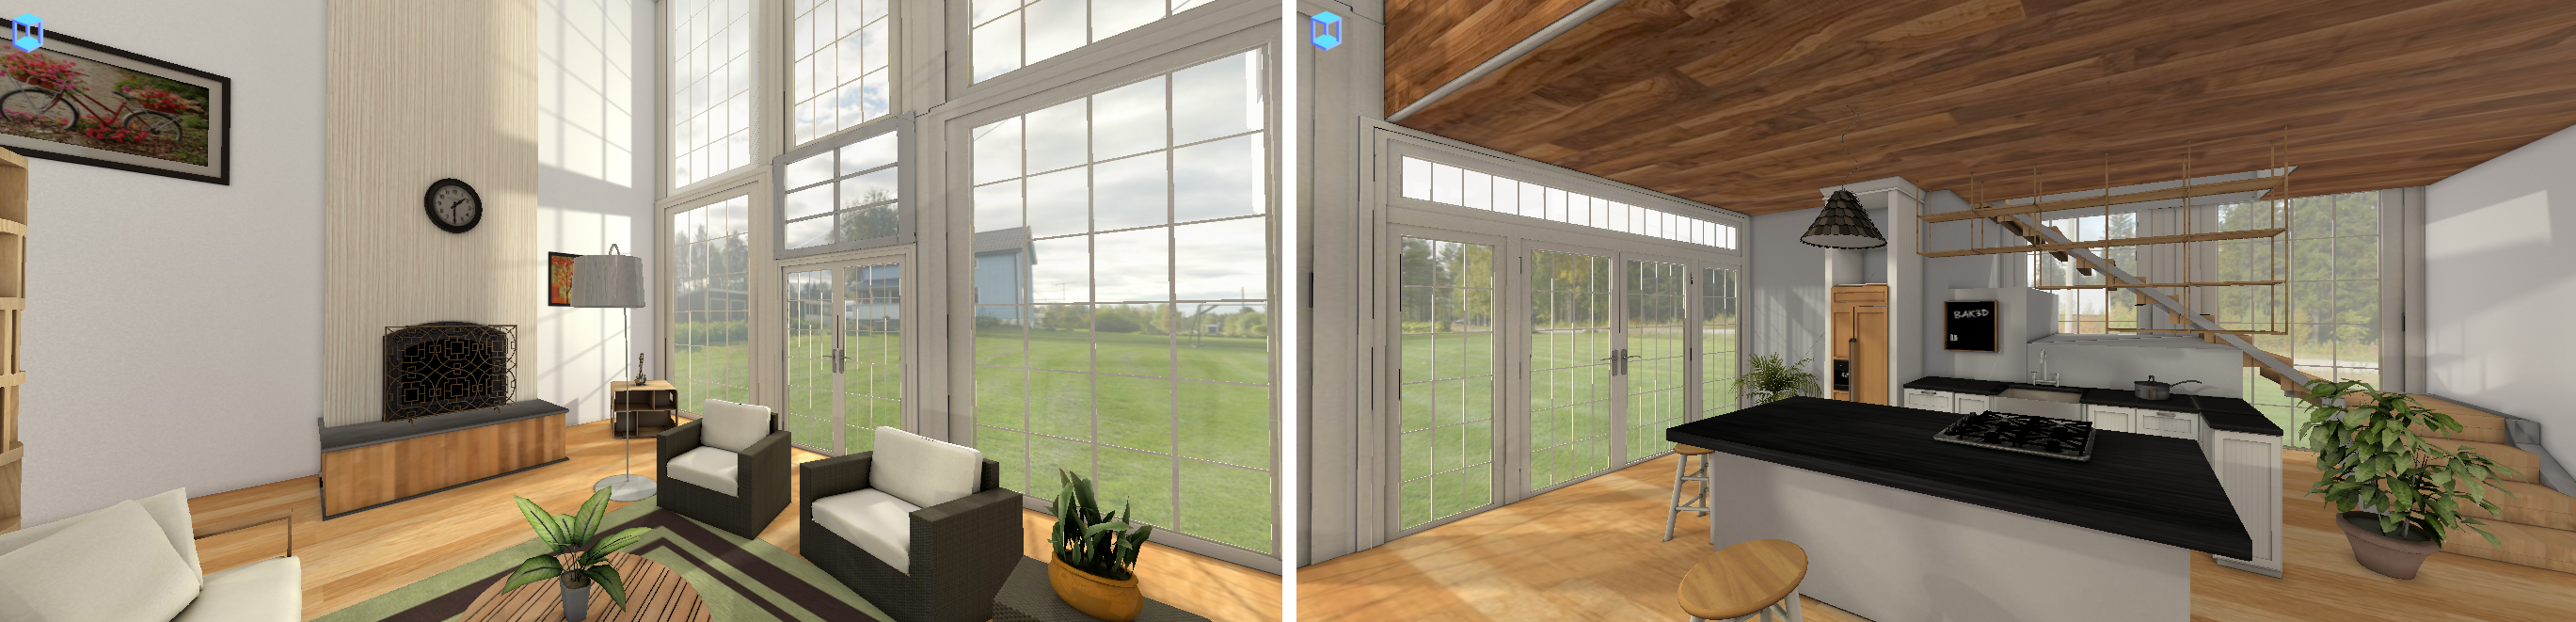
\includegraphics[width=0.99\linewidth]{images/chapter_navigazione_scena/vis_sin_des.png}\hfill
 \caption[Esempio 1 di osservazione virtuale]{Sguardo dell'osservatore virtuale rivolto verso sinistra e verso destra.}
 \label{fig:navigazione_scena_vis_sin_des}
\end{figure}
\begin{figure}[h]
 \centering
 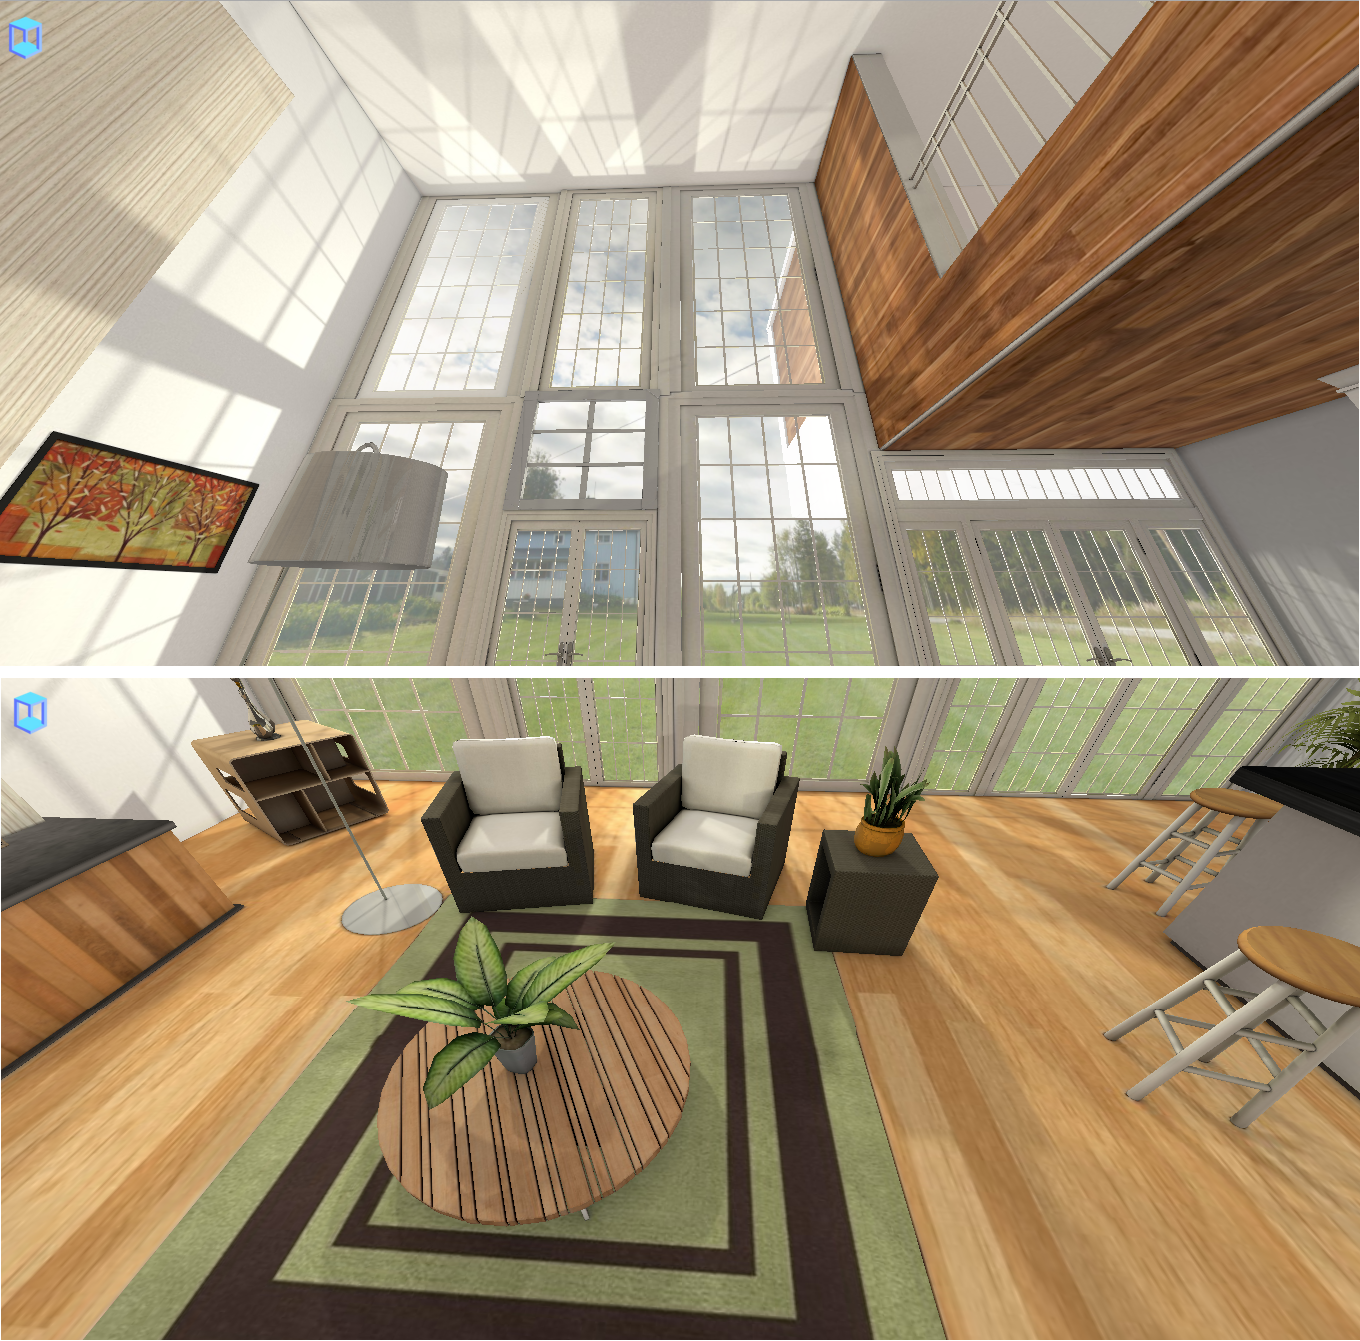
\includegraphics[width=0.80\linewidth]{images/chapter_navigazione_scena/vis_alta_bassa.png}\hfill
 \caption[Esempio 2 di osservazione virtuale]{Sguardo dell'osservatore virtuale rivolto verso l'alto e verso il basso.}
 \label{fig:navigazione_scena_vis_alta_bassa}
\end{figure}
\\
Quando questa modalità viene avviata, il menu in alto a destra (visibile in figura \ref{fig:navigazione_scena_navigator_int}) ed il puntatore del mouse vengono nascosti per permettere una navigazione a schermo intero.
\\
L’osservatore virtuale che si muove nella scena è costituito da un oggetto 3D a cui è associata una camera prospettica.
\\
L’oggetto 3D rappresenta il “corpo” dell’osservatore; lo spostamento di questo oggetto all’interno dello spazio consente di ricreare una passeggiata virtuale nella scena.
In particolare permette di camminare, saltare e, quando possibile, salire o scendere gli oggetti (es.scale o un divano) nell’ambiente.
\\
La camera invece rappresenta gli “occhi” dell’osservatore; è possibile ruotare la camera in una direzione compatibile con quelle dalla testa umana. 
\\
Questo ha permesso di dare l’illusione all’utilizzare del servizio di navigazione che lui stesso stia visitando l’ambiente.
In particolare viene permesso di osservare la scena da una altezza di 1.80 metri. Questa modalità risulta molto utile per permettere all’utilizzatore di farsi una idea concreta dello spazio occupato dalla scena creata.
\\
Inoltre esattamente come nei videogiochi, viene permesso all’utente di mettere in pausa la navigazione.
Quando questo avviene, i controlli di movimento vengono bloccati e torna visibile il menu ed il puntatore del mouse. Questo permette all’utente di scegliare se cambiare modalità di navigazione  oppure continuare con quella in prima persona.
\begin{figure}[htb]
 \centering
 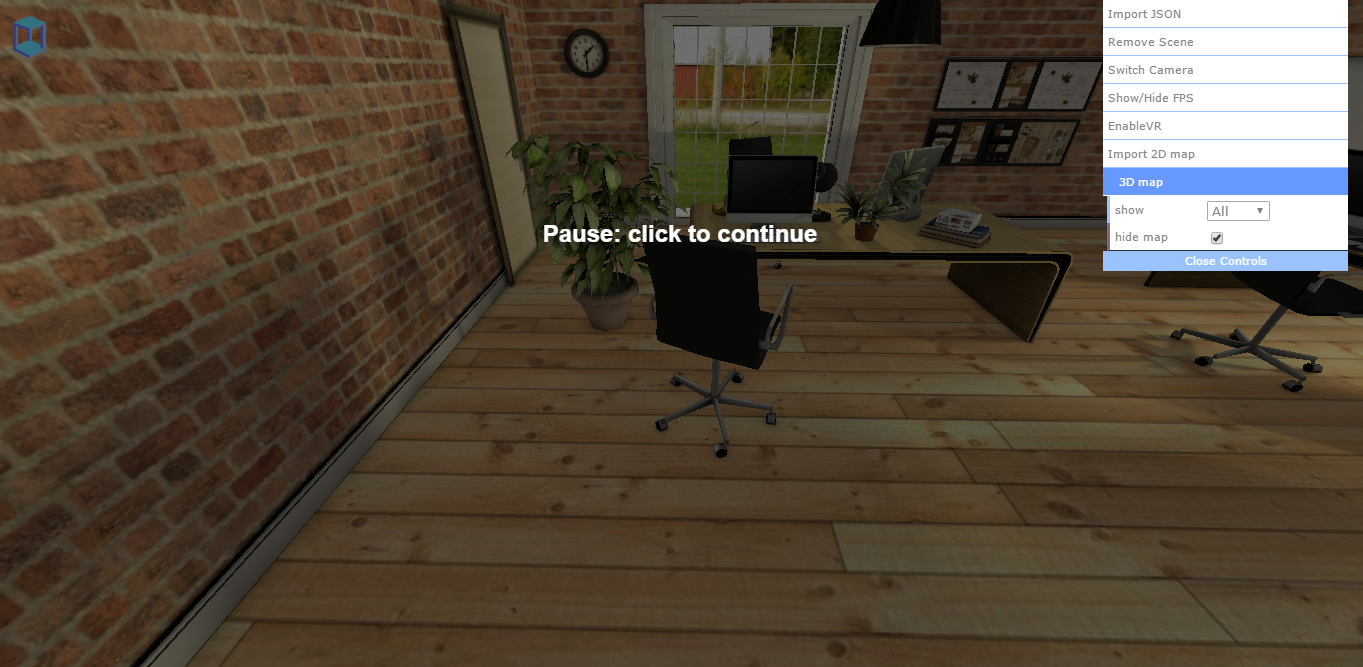
\includegraphics[width=1\linewidth]{images/chapter_navigazione_scena/navigator_pause.png}\hfill
 \caption[Navigazione in pausa.]{Navigazione in pausa.}
 \label{fig:navigazione_scena_navigator_pause}
\end{figure}
\newpage
Quando viene visitata una abitazione, la navigazione in prima persona, permette all’utente di valutare la grandezza delle stanze in rapporto all’osservatore virtuale inserito nella scena. Questo permette di fornire all’utente una idea migliore della larghezza e dell’altezza di ogni stanza creata.
\\
In particolare nel presente lavoro di tesi vengono navigate scena fotorealistiche prodotte dal sistema creato. In queste scene sono inserite informazioni di luci ed ombre estremamente realistiche.
\\
Un architetto potrebbe utilizzare questo servizio per permettere agli acquirenti di una casa di visitarne gli interni ancora prima che essa sia costruita.
Gli acquirenti in questo modo possono farsi una idea estremamente precisa dello spazio disponibile e di quanto le stanze siano illuminate dalla luce solare.
Informazione fondamentale anche per l’architetto durante la progettazione di un appartamento.
\\
Inoltre l’elevato grado di realismo delle luci create permetterebbe all’architetto di valutare la luce ambientale entrante in una stanza anche quando ci sono ostacoli di fronte alla finestra da cui entra la luce (es. un palazzo). Sarebbe sufficiente ricreare l’ostacolo nella scena virtuale e poi valutare la luce proiettata nella stanza con il servizio di navigazione.
\\
Inoltre al fine di dare all’utente un’idea ancora più precisa degli spazi creati sono state effettuate delle sperimentazioni tramite visori di realtà virtuali.
\\ 
Nel paragrafo seguente verrà spiegato come essi sono stati utilizzati.

\subsection{Navigazione in realtà virtuale}
Nel navigatore è disponibile la funzionalità che permette la navigazione della scena tramite la realtà virtuale.
\\
Questa modalità permette di annullare per intero quello che l’utente vede dell’ambiente reale, dandogli la sensazione di trovarsi in un altro luogo, in questo caso la scena realizzata in Three.js \cite{realtavirt}.
\\
In particolare questa modalità permette la visione stereoscopica dell’ ambiente virtuale.
Esistono diversi dispositivi dedicati alla realtà virtuale, prodotti con notevoli potenzialità dal punto di vista dell’intrattenimento e che nei giorni d’oggi vengono soprattutto utilizzati all’interno dell’industria videoludica.
\\
In particolare in questo lavoro di tesi sono stati sperimentati due tipi di visori 3D: l’Oculus Rift ed il Google Cardboard. 
L’Oculus Rift è un visore steroscopico di realtà virtuale sviluppato dalla società Oculus VR.
\begin{figure}[htb]
 \centering
 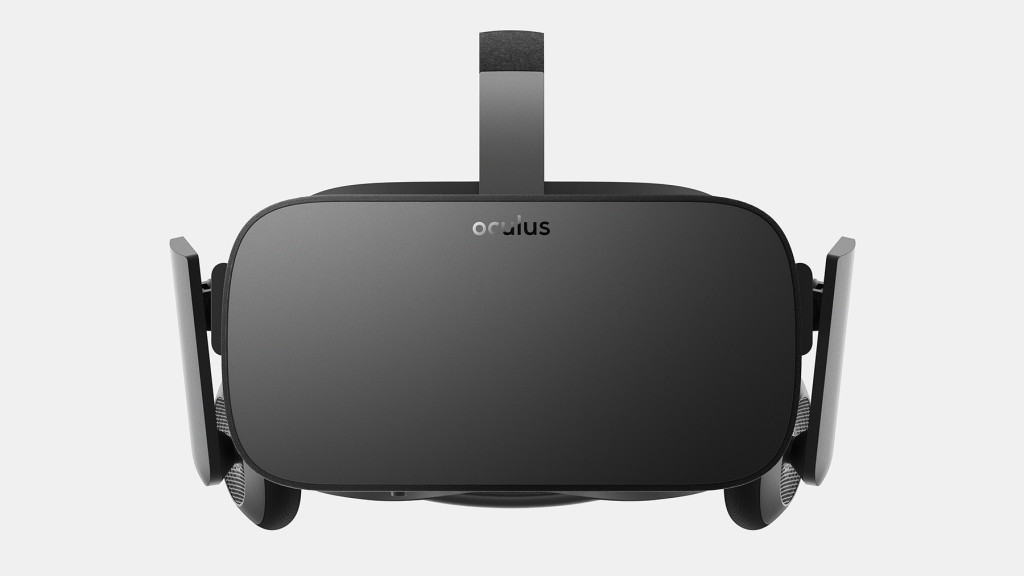
\includegraphics[width=0.8\linewidth]{images/chapter_navigazione_scena/oculus.jpg}\hfill
 \caption[Il visore Oculus Rift.]{Il visore Oculus Rift.}
 \label{fig:navigazione_scena_navigator_oculus}
\end{figure}
\\
Esso permette la visione stereoscopica di un ambiente virtuale ad una qualità elevata tramite due display che girano ad una risoluzione HD di 2160x1200 (1080x1200 per occhio) con un refresh rate di 60HZ \cite{oculus_caratt}.
\\
Inoltre permette un campo di visione di 100 gradi in orizzontale, il massimo raggiunto da visori di questo tipo. Questo permette all’utilizzatore del dispositivo di non osservare eccessive zone scure, dovute al rivestimento del sensore, intorno ai bordi del display. 
\\
Inoltre traccia le informazioni di posizione e rotazione della testa dell’utilizzatore permettendo di modificare il volume di vista della camera in base a questi due parametri.
\\
Queste informazioni vengono calcolate mediante l’utilizzo di diversi sensori come il giroscopio, l’accelerometro ed il magnetometro che permettono di determinare il movimento della testa dell’utente nel mondo reale e sincronizzarla con la vista virtuale dell’utente nell’ambiente proiettato.
\\
Durante questo lavoro di tesi, è stata studiata una sua versione prototipale del sensore ed ha permesso di sperimentale una ottima qualità durante la visione stereoscopica di una scena virtuale. Purtroppo però il sensore non risultava compatibile con le librerie Three.js create appositamente per permetterne l'utilizzo in ambiente web.
\\
Durante il lavoro di tesi sono stati valutati i benefici e gli svantaggi nell’utilizzo di questo dispositivo. Tra i benefici riscontrabili c’è l’elevata qualità di visione virtuale, tra gli svantaggi è doverose segnalare l’ elevato costo; il prodotto uscirà ufficialmente nel mercato a Marzo 2016 e costerà 699 euro \cite{oculus_prezzo}.
Un elevato costo che difficilmente potrà essere sostenuto da qualsiasi tipologia di utente.
\\
Inoltre questo tipo di visore risulta compatibile solamente su calcolare di alte prestazioni; l’architettura minima richiesta è la seguente: \cite{oculus_pc_compat}
\begin{itemize}
\item Scheda grafica: NVIDIA GTX 970 / AMD R9 290.
\item Processore: Intel i5-4590.
\item Memoria: 8GB RAM.
\item Output: HDMI 1.3 video output.
\item Input: 3 porte USB 3.0 più una porta USB 2.0.
\item Sistema operativo: Windows 7 SP1 64 bit o successivo.
\end{itemize}
Inoltre questo visore non risulta compatibile con i sistemi operativi OS X e Linux.\cite{oculus_mac}
\\
L’Oculus Rift non si adattava bene ad essere utilizzato per questo elaborato proprio per le prestazioni di utilizzo richieste. Fondamentale in questo lavoro di tesi infatti è la fruibilità di queste scene su qualsiasi tipo di architettura anche su quelle con prestazioni basse.
\\
Sarebbe quindi inutile inserire una funzionalità come quella della realtà virtuale tramite il sensore Oculus se poi  essa non può essere fruita in tale contesto.
\\
Per questo motivo, nel presento lavoro di tesi è stato invece utilizzato il visore stereoscopico Google Cardboard sviluppato da Google \cite{cardboard}.
\\
\begin{figure}[htb]
 \centering
 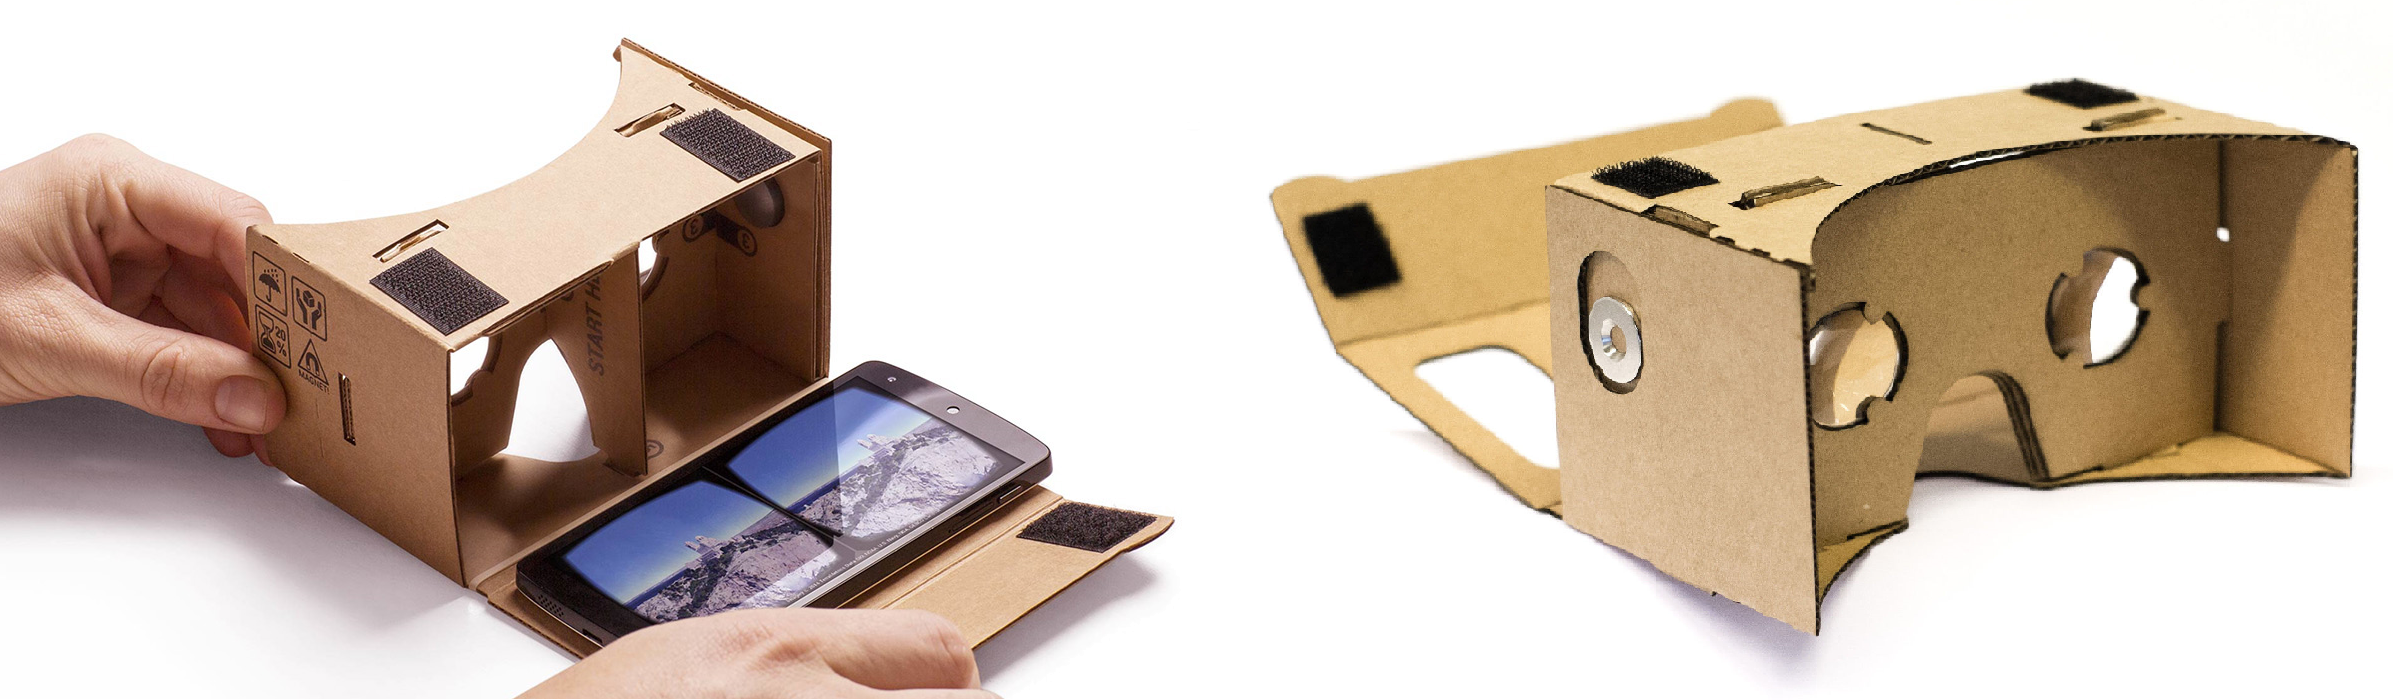
\includegraphics[width=1\linewidth]{images/chapter_navigazione_scena/cardboard.png}\hfill
 \caption[Il visore Google Cardboard.]{Il visore Google Cardboard.}
 \label{fig:navigazione_scena_navigator_oculus}
\end{figure}
\\
Questo visore è costituito da semplici componenti a basso costo: Cartone da ritagliare, Due lenti con distanza focale di 45 mm (che permettono un angolo di visione di 90 gradi), un magnete e degli elastici.
\\
Le parti acquistate devono essere assemblate insieme dall’utilizzatore al fine di costruire il Cardboard (figura \ref{fig:navigazione_scena_navigator_cardboard_pezzi}).
\begin{figure}[htb]
 \centering
 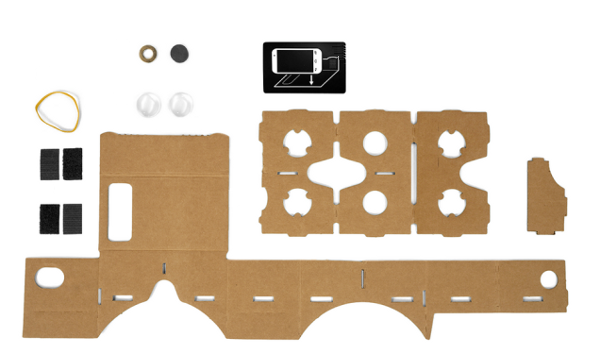
\includegraphics[width=0.8\linewidth]{images/chapter_navigazione_scena/cardboard_pezzi.png}\hfill
 \caption[Le componenti del CardBoard.]{Le componenti del CardBoard.}
 \label{fig:navigazione_scena_navigator_cardboard_pezzi}
\end{figure}
\\
Una volta costruito il visore di cartone è necessario inserire lo smartphone all’interno della fessura presente in esso. Lo smartphone funge infatti da display delle immagini da visualizzare.
\\
Le immagine proiettate dal cellulare sulle due lenti permettono la visione stereoscopica (3D).
Inoltre è possibile tracciare le informazioni di posizione e rotazione della testa dell’utilizzatore sfruttando il giroscopio e l’accelerometro del cellulare. 
\\
Il magnete invece permette di sfruttare il magnetometro del cellulare al fine di interagire con l’applicazione cardboard avviata.
\\
Questo visore può essere acquistato per pochi euro e, vista la diffusione degli smartphone, è accessibile praticamente ad ogni utente. 
\\
Inoltre è compatibile con praticamente tutti gli smartphone, anche con quelli di prestazioni basse e non necessita alcune installazione, a differenza dell’ Oculus Rift.
Nel presente contesto di lavoro ha permesso la fruizione stereoscopica di una scena fotorealistica realizzata dal sistema creato.
Il navigatore, quando viene avviata questa modalità, effettua delle operazioni atte a permettere la fruizione in 3D della scena. 
\\
La canvas, in cui viene disegnata la scena, viene divisa a metà in larghezza. La metà sinistra e  quella destra rappresentano di fatto due immagini del medesimo ambiente riprese alla stessa distanza ma scostate lateralmente con uno scarto pari alla distanza binoculare (5-7,5cm).
\begin{figure}[htb]
 \centering
 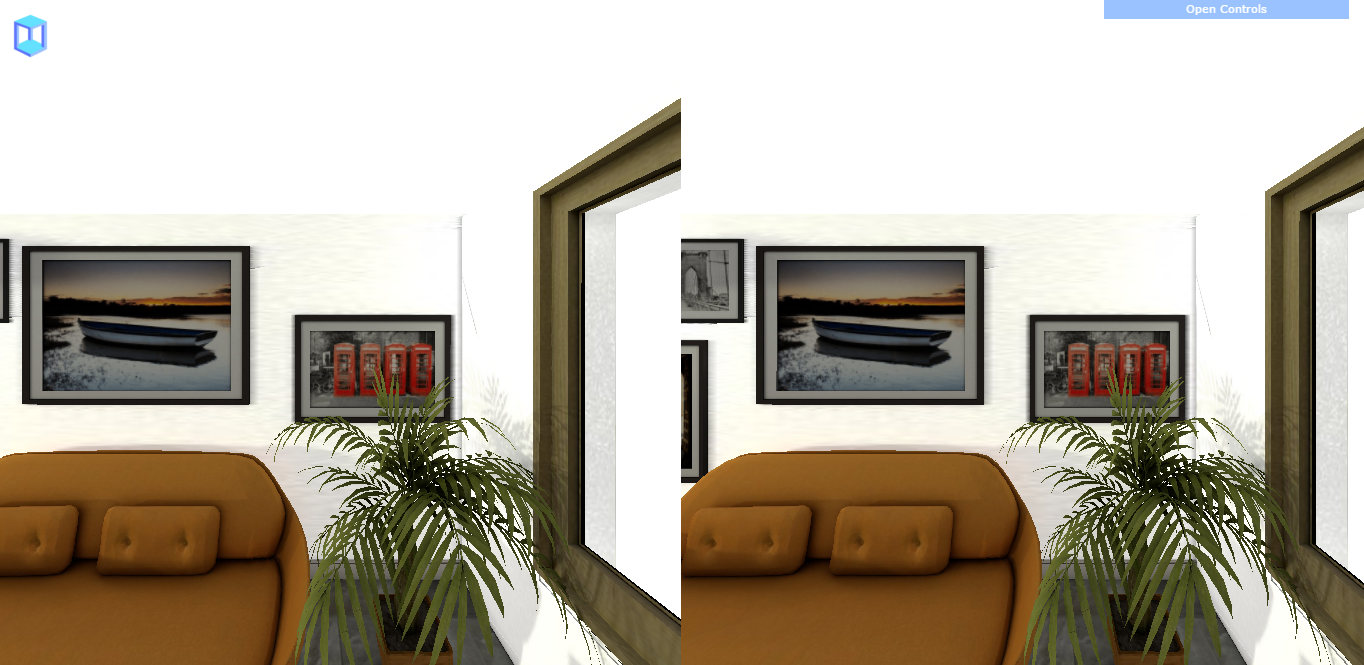
\includegraphics[width=1\linewidth]{images/chapter_navigazione_scena/immag_virt.png}\hfill
 \caption[Visione stereoscopica.]{La visione stereoscopica.}
 \label{fig:navigazione_scena_navigator_immag_virt}
\end{figure}
\\
Per ogni ciclo di render vengono disegnate due immagini di questo tipo che, tramite l’utilizzo delle lenti presenti nel visore, permettono la visione stereoscopica.
\\
Inoltre sono stati sfruttati l’accelerometro ed il giroscopio per permettere di modificare la vista sulla scena virtuale in maniera proporzionale a come l’utente muove la testa.
\\
Quando viene avviata questa modalità, la visione passa in prima persona, ma a differenza del paragrafo \ref{sec:chapter_navigazione_scena_caratt_navigat_navig_alto}, i controlli utilizzati sono differenti.
\\
Non è possibile infatti sfruttare i normali controlli in prima persona in quanto lo smartphone è inserito all’interno del visore e non è possibile interagire con esso tramite comandi touch o tramite tastiera.
\\
Durante questa modalità il movimento avviene automaticamente in avanti secondo la direzione di osservazione, quest’ultima viene modificata mediante l’utilizzo dell’oscilloscopio del cellulare.
Il movimento automatico in avanti avviene ad una velocità tale da simulare una normale passeggiata all’interno di una abitazione.
\\
I dettagli implementativi di come è stato realizzata questa modalità del navigatore verrano descritti nel paragrafo \ref{sec:chapter_navigazione_scena_implementazione}.

\subsection{Mappa di navigazione}
\label{sec:caratteristiche_navigatore_mappa}

Quando viene avviata la navigazione in prima persona è possibile attivare o disattivare la mappa di navigazione.
La mappa permette di osservare la scena caricata tramite una vista aerea.
\\
Essa consente infatti all’utilizzatore di orientarsi all’interno dell’ambiente ed è particolarmente utile in scene di medie e grandi dimensioni.
\\
Mappe di questo tipo vengono utilizzate soprattutto nei videogiochi.
In particolare all’interno della mappa viene disegnata l’area navigabile della scena e viene disegnato il giocatore, identificabile tramite un indicatore (visibile in figura \ref{fig:navigazione_scena_map_lost_odissey}). 
L’indicatore risulta utile per mostrare la direzione in cui osserva il personaggio.
\\
Durante il movimento del giocatore nella scena, l’indicatore del personaggio rimane fisso al centro della mappa, mentre l’ambiente disegnato intorno ad esso si muove in base allo spostamento effettuato.
\\
La mappa quindi segue il movimento del giocatore all’interno della scena mostrando di volta in volta l’ambiente intorno ad esso. 
Il fatto che il giocatore sia centrato nella mappa permette di ottenere una visione completa dell’ambiente circostante tramite una vista aerea, vista utile ai fini dell’orientamento.
\\
\begin{figure}[htb]
 \centering
 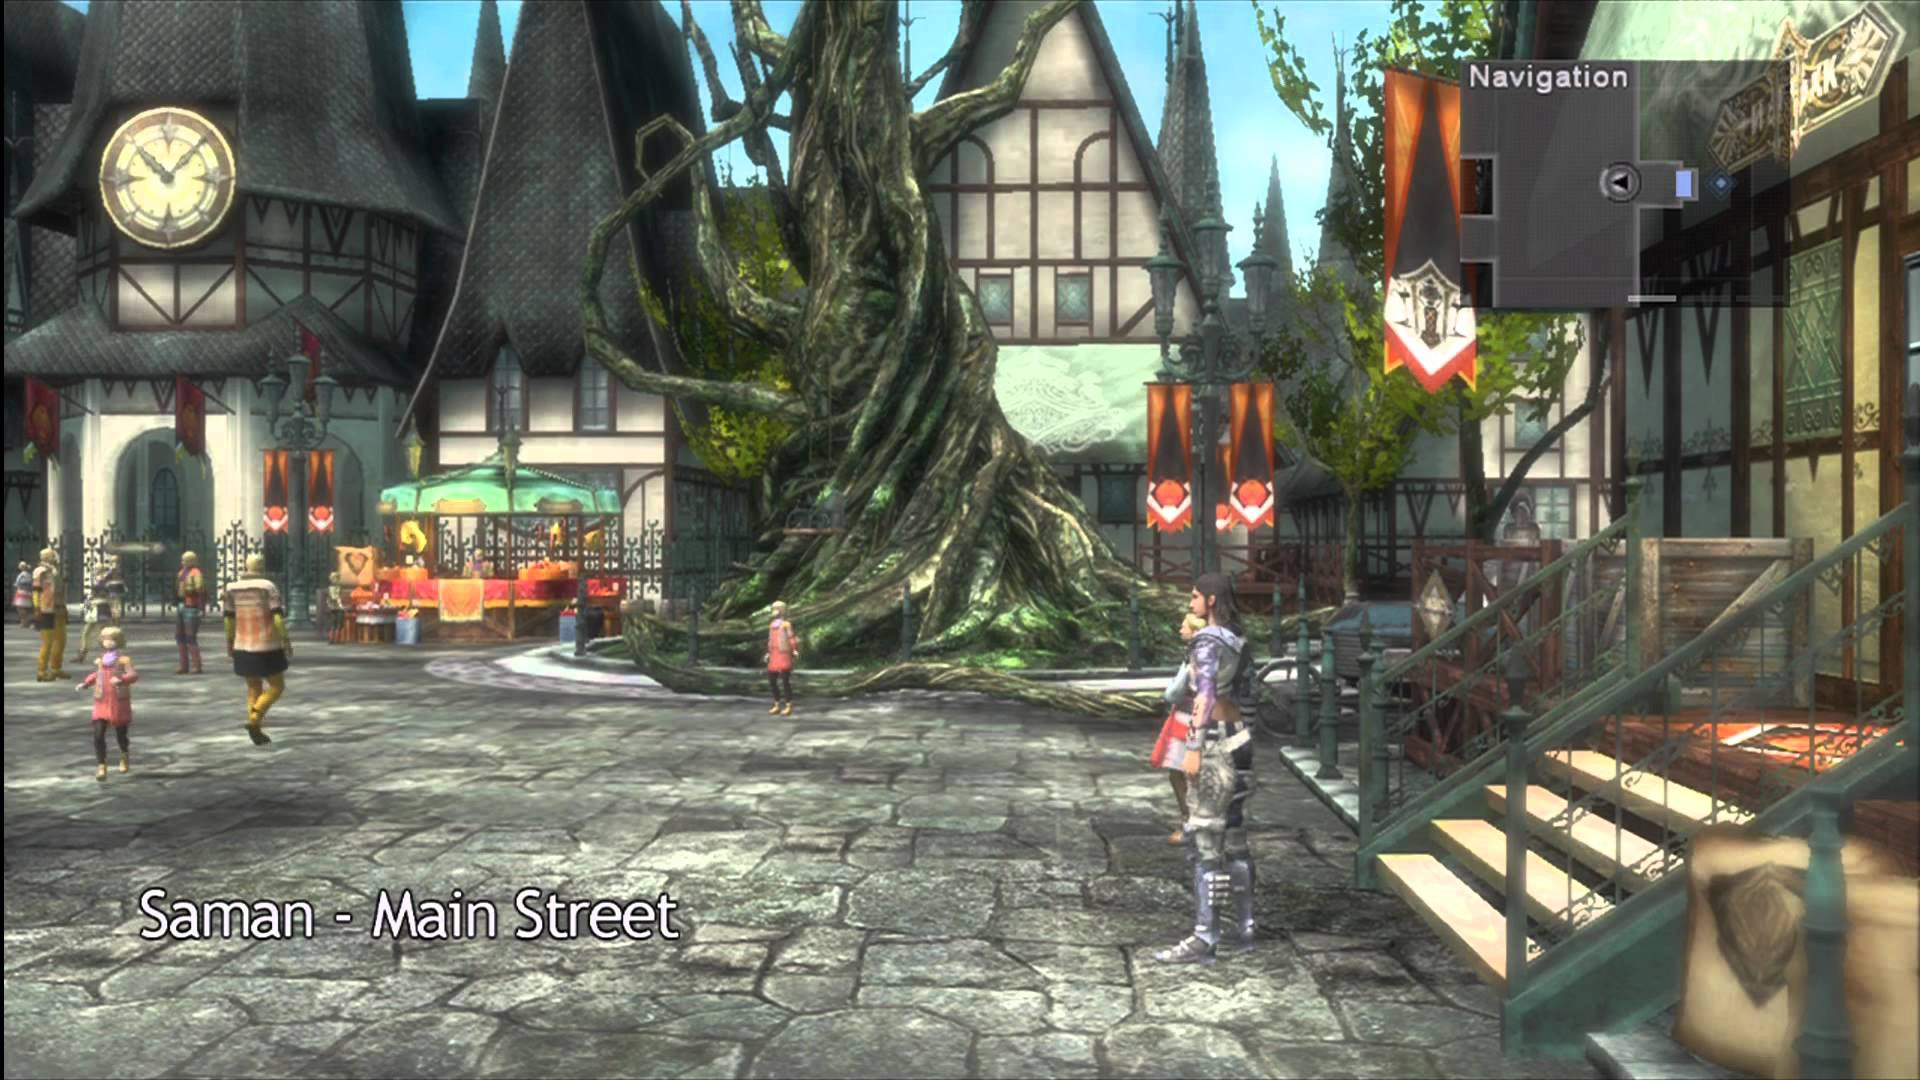
\includegraphics[width=1\linewidth]{images/chapter_navigazione_scena/map_lost_odissey.jpg}\hfill
 \caption[Mappe nei videogiochi.]{Mappa proveniente dal videogioco \emph{Lost Odissey} (2008).}
 \label{fig:navigazione_scena_map_lost_odissey}
\end{figure}
\\
In questo lavoro di tesi è stato preso spunto dalle mappe utilizzate nei videogiochi per la realizzazione di una mappa visualizzabile durante la navigazione delle scene fotorealistiche create.
\\
Esattamente come per quelle dei videogiochi, la mappa disegna l’area navigabile della scena e disegna l’osservatore virtuale tramite un indicatore blu a forma di chiocciola. In particolare la punta della chiocciola indica la direzione di movimento dell’osservatore.
\\
L’ambiento disegnato sulla mappa si muove in base allo spostamento effettuato dall’osservatore e l’indicatore viene mantenuto fisso al centro della mappa.
\\

Nella mappa creata risulta possibile scegliere la modalità con cui viene disegnato l’ambiente della mappa:
\begin{itemize}
\item Disegno dell’ intera scena 3D.
\item Disegno di mura e/o pavimenti della scena 3D.
\item Disegno, tramite lettura di un apposito file JSON, dell’ ambiente in 2D.
\end{itemize}

La mappa in tutte e tre le modalità viene costruita tramite un differente renderer da quello utilizzato per disegnare la scena. 
\\
Ad esso è associata una canvas in cui viene renderizzato l’ambiente ed il puntatore che rappresenta l’osservatore. Gli oggetti da renderizzare vengono inseriti all’interno di una scena creata appositamente per contenere gli elementi mostrati dalla mappa.
\\
Nella prima modalità, all’interno della mappa viene renderizzato lo stesso ambiente disegnato dal renderer principale.
\\
In particolare viene renderizzata la porzione di scena contenuta nel volume di vista di una camera posizionata sopra all’osservatore virtuale e direzionata verso di esso.
La camera segue i movimenti dell’osservatore, mantenendo l’osservatore al centro del volume di vista renderizzato.
\begin{figure}[htb]
 \centering
 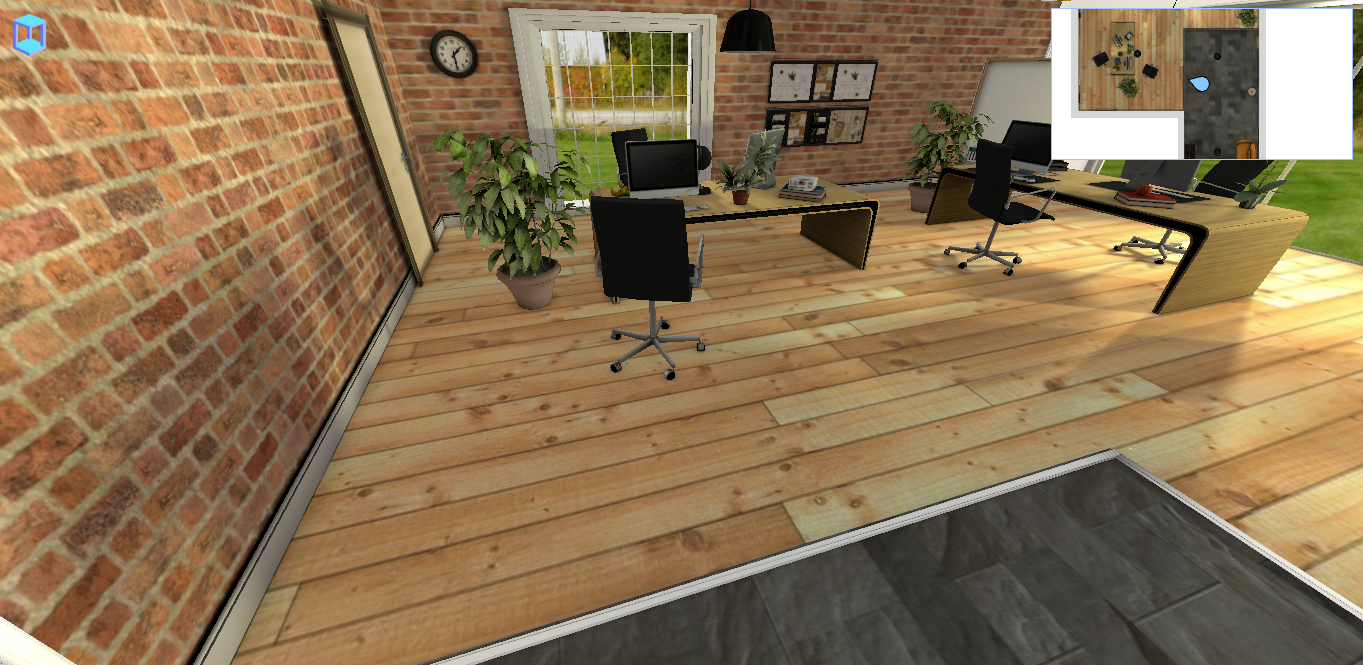
\includegraphics[width=1\linewidth]{images/chapter_navigazione_scena/map_3d.png}\hfill
 \caption[Mappa completa della scena.]{Mappa completa della scena.}
 \label{fig:navigazione_scena_map_3d}
\end{figure}
Siccome la scena disegnata nella mappa è 3D, non è possibile utilizzare una camera prospettica. Viene invece utilizzata una camera che permette una proiezione ortografica in cui gli oggetti non diventano più piccoli mano a mano che si allontanano da essa.
\\
Questo permette di mostrare una mappa bidimensionale, vista dall’alto, della scena creata.
La procedura appena descritta permette di ottenere una mappa che ricrea fedelmente l’ambiente circostante, compreso l’arredamento inserito nell’appartamento.
\\
La tecnica però risulta inefficiente quando viene renderizzata una scena di grandi dimensioni. Essa infatti appesantisce l’applicazione in quanto durante la navigazione viene renderizzata la stessa scena due volte.
\\
Una volta nella canvas di dimensioni pari allo schermo in cui viene mostrata la navigazione e l’altra volta sulla canvas ridotta in cui è mostrata la mappa. Nonostante le ridotte dimensioni, la renderizzazione di questa comporta rallentamenti nella fluidità quando la scena da disegnare è costituita da molti oggetti.
\\
Rallentamenti che per hardware di basse prestazione possono portare ad una diminuzione degli fps tale da rendere di fatto impossibile la navigazione.
\\
Per questo motivo è possibile decidere di renderizzare sulla mappa solamente i muri e/o i pavimenti dell’ appartamento da renderizzare.
\\
Nell’editor, agli oggetti muro e pavimento viene assegnato un attributo differente che permette di distinguere gli uni dagli altri, esso viene riportato all’interno del formato di scambio.
\\
Quindi nella mappa è possibile renderizzare solamente questi due tipi di strutture, scartando tutti gli altri oggetti come quelli dell’arredamento. Questo permette di ridurre notevolmente il carico computazionale del render. 
\\
Gli oggetti pavimento sono infatti dei semplici oggetti piano di colore grigio chiaro ed i muri costituiti da Shape Geometry vengono trasformati in piani grigi visti dall’alto al fine di risultare più leggeri per il ciclo di render. Ai piani creati viene assegnato un materiale MeshBasic che non dipende dalla luce, questo perchè nella scena della mappa non sono presenti fonti luminose.
\begin{figure}[htb]
 \centering
 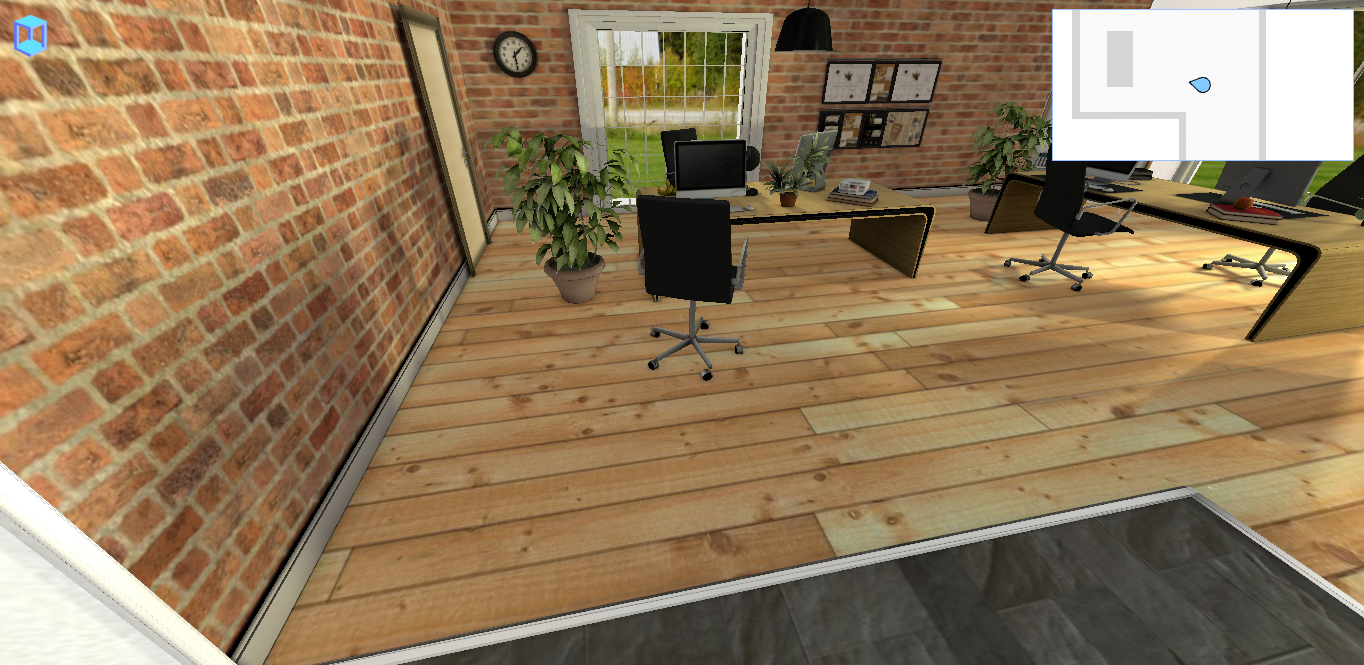
\includegraphics[width=1\linewidth]{images/chapter_navigazione_scena/map_2d_json.png}\hfill
 \caption[Mappa con soli muri e pavimenti.]{Mappa con soli muri e pavimenti.}
 \label{fig:navigazione_scena_map_2d_json}
\end{figure}

Questa mappa creata risulta estremamente efficiente anche su calcolatori di basse prestazioni. Essa risulta particolarmente adatta agli utenti a cui interessa che nella mappa sia mostrata solamente la struttura dell’appartamento e non l’arredamento.
\\

Infine il navigatore permette la creazione di una mappa 2D creata ad hoc per la scena tramite un file \emph{.json}.
Nel file \emph{.json} è descritta la struttura dell’intero edificio creato, quindi contiene le informazioni dei pavimenti, dei muri e del soffitto.
\\
Questo file può essere scritto a mano dall’utilizzatore oppure può essere creato da un’applicazione in sviluppo nel laboratorio di tesi che permette la creazione di muri, pavimenti e soffitto tramite una semplice interfaccia creata appositamente per svolgere questo compito.
\\
Il navigatore legge questo formato di scambio ed identifica le informazioni sui muri e sui pavimenti. Le informazioni sul soffitto vengono invece scartate altrimenti esso coprirebbe l’abitazione interna osservata nella mappa dall’alto.
Una volte ottenute le informazioni necessarie vengono creati dei piani a due dimensioni che rappresentano i muri ed i pavimenti visti dall’alto.
\\
Anche questa mappa risulta particolarmente efficiente in quanto le geometrie da renderizzare risultano molto semplici.
\\
L’utente può ricorrere a questo tipo di mappa quando i muri o i pavimenti non hanno assegnato l’attributo corretto che permette la creazione automatica della mappa con soli muri e pavimenti, oppure quando i risultati ottenuti dalla creazione automatica non lo aggradano e quindi preferisce crearne una personalmente.
\begin{figure}[htb]
 \centering
 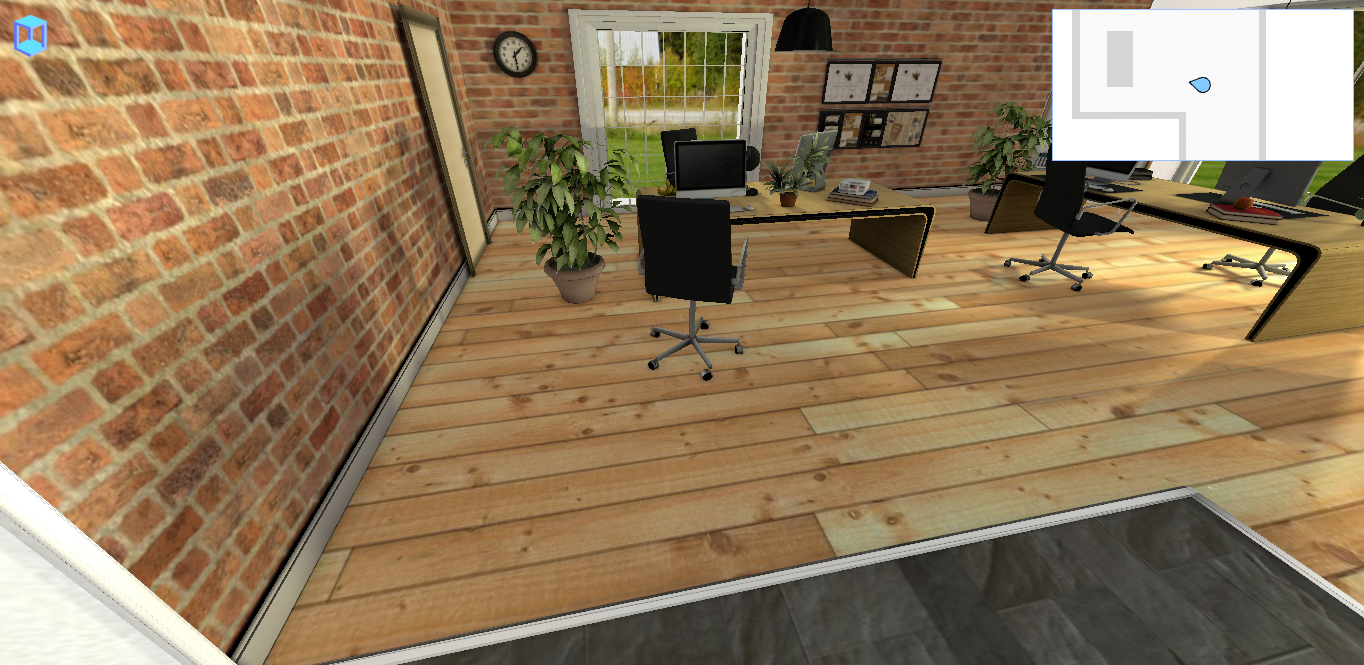
\includegraphics[width=1\linewidth]{images/chapter_navigazione_scena/map_2d_json.png}\hfill
 \caption[Mappa creata dal file JSON4.]{Mappa creata dal file JSON4 in cui viene disegnata anche la scrivania.}
 \label{fig:navigazione_scena_map_2d_json}
\end{figure}